\maketitle
\setcounter{page}{1}
\tableofcontents
\newpage
\pagenumbering{arabic}
\section{Theorie}
Ziel des Versuchs ist die Untersuchung der Suszeptibilität $\chi$ paramagnetischer Oxide
von Selten-Erd-Verbindungen.
\subsection{Theorie des Paramagnetismus}
\label{sec:1.1}
Der Paramagnetismus ist ein Quantenphysikalisches Phänomen,
von daher muss eine Beziehung für die Suszeptibilität auch aus Quantenphysikalischen
Überlegungen folgen.\\
\noindent
Für die Magnetische Flussdichte $\vec{B}$ gilt in Materie die Beziehung
\begin{equation}
  \vec{B} = \mu_0 \vec{H} + \vec{M}
\end{equation}
mit Magnetfeldkonstante $\mu_0$, magnetischer Feldstärke $\vec{H}$ und Magnetisierung $\vec{M}$.
Die Magnetisierung entsteht auf atomarer Ebene aufgrund magnetischer Momente. Sie berechnet sich zu
\begin{equation}
  \vec{M} = \mu_0 \chi \vec{H},
\end{equation}
hängt also von der selbst Temperatur- und Magentfeldabhängigen Subszeptibilität $\chi$ ab.
Quelle des Paramagnetismus ist der nicht verschwindende Gesamtdrehimpuls bestimmter Atome,
der eine Ausrichtung der magnetischen Momente zu einem äußeren Feld bewirkt. Der Gesamtdrehimpuls $\vec{J}$
eines Atoms ist näherungsweise die Vektorsumme aus Gesamtbahndrehimpuls $\vec{L}$
und dem Gesamtspin $\vec{S}$ der Elektronen, die sich jeweils aus den Vektorsummen der
Einzelanteile aller Elektronen zusammensetzen. Für die magnetischen Momente der beiden
Drehimpulsanteile folgt aus Quantenphysikalischen Überlegungen nun:
\begin{align}
  | \vec{\mu}_L | &= \mu_B \sqrt{L(L+1)} \\
  | \vec{\mu}_S | &= \mu_B \, g_{S} \sqrt{S(S+1)},
\end{align}
wobei $L$ und $S$ die Quentenzahl des jeweiligen Drehimpulses, $\mu_\symup{B} \coloneq
1/2 \, e_0 m_0^{-1} \hbar$ das $\textsc{Bohrsche}$ Magneton und $g_S$ das gyromagentische
Verhältnis sind. Für den Betrag des Gesamtmoments folgt aus geometrischen Überlegungen
dem Cosinussatz und der Quantenmechanik weiter:
\begin{equation}
  | \vec{\mu}_J | \approx \mu_B \sqrt{J(J+1)} \, g_J,
\end{equation}
wobei $g_J$ der $\textsc{Landé}$-Faktor
\begin{equation}
  g_J = \frac{ 3 J(J+1) + ( S(S+1) - L(L+1) ) }{ 2 J(J+1) }
  \label{eqn:1}
\end{equation}
ist. Als letztes Ergebnis aus der Quantenmechanik ist die Richtungsquantelung wichtig.
Sie besagt, dass nicht beliebige Winkel zwischen $\vec{\mu}_J$ und $\vec{H}$ möglich sind,
sodern nur solche, bei denen die $z$-Komponente des Momentes die Beziehung
\begin{equation}
  \mu_{J, \, z} = - \mu_B \, \g_J \, m
  \label{eq:1}
\end{equation}
erfüllt, wobei $m$ die ganzzahlige Orientierungsquentenzahl bezeichnet. Für das
magnetische Moment folgen daher $2J+1$ mögliche Winkel relativ zu $\vec{H}$. Jedem
dieser Winkel ist nun eine potentielle Energie zugeordnet. Aus \eqref{eq:1} folgt
mit statistischen Methoden sowie der ebenfalls statistischen $\textsc{Boltzmann}$-Verteilung
letztlich für $\chi$:
\begin{equation}
  \chi = \frac{\mu_0 \, \mu_B^2 \, g_J^2 \, N \, J(J+1)}{3 \, k_B \, T}
  \label{eqn:3}
\end{equation}
mit $\textsc{Boltzmann}$-Konstante $k_B$ und der Anzahl der Momente pro Volumeneinheit $N$.
Man erkennt die $T^{-1}$ Proportionalität der Suszeptibilität, die auch als $\textsc{Curiesches}$
Gesetz des Paramagnetismus bekannt ist.\\
\noindent
Verantwortlich für die besonders starke Ausprägung des Paramagnetismus bei Seltenen-Erden
ist das Vorhandensein von einer ungesättigten 4f-Schale, die, da tief in der 6s-Schale liegend, auch noch
bei ihren Ionen vorhanden sind. Aussagen über diese Konstellation und die Konsequenzen
für den Gesamtdrehimpuls erlauben die $\textsc{Hundschen}$-Regeln:
\begin{itemize}
  \item[1.] Der Gesamtspin $\vec{S}$ nimmt den maximal möglichen Wert an, den das $\textsc{Pauli}$-Prinzip erlaubt.
  \item[2.] Der Gesamtbahndrehimpuls $\vec{L}$ nimmt den nach 1 und dem $\textsc{Pauli}$-Prinzip möglichen
  maxmimalen Wert an.
  \item[3.] Für den Gesamtdrehimpuls $\vec{J}$ gilt:
  \begin{equation}
  \vec{J} =
    \begin{cases}
      \vec{L} - \vec{S} \; , \, \text{Schale weniger als halb besetzt} \\
      \vec{L} + \vec{S} \; , \, \text{Schale mehr als halb besetzt}
    \end{cases}
  \end{equation}
\end{itemize}
\subsection{Messmethode zur Bestimmung der Suszeptibiliät}
\label{1.2}
\begin{figure}
  \centering
  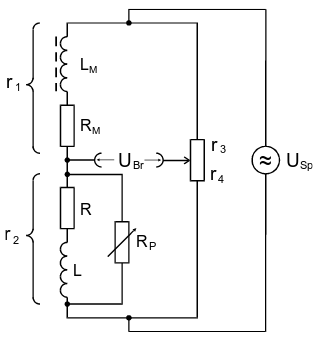
\includegraphics[scale = 0.5]{Bruecke.png}
  \caption{Aufbau der verwendeten Brückenschaltung\cite{anleitung}.}
  \label{abb:1}
\end{figure}
Zur Messung der Suszeptibilität bietet sich eine Brückenschaltung wie in Abbildung \ref{abb:1}
an. Die Bestimmung der Suszeptibilität finden nun über zwei Spulen statt, deren Induktivitäten
abgeglichen werden und von denen eine mit der Probe befüllt wird. Es ergeben sich nun zwei Grundsätzliche
Möglichkeiten:
\begin{itemize}
  \item [1.] Zu Anfang wird die Brückenschaltung über ein Potentiometer
  so abgeglichen, dass keine Spannung mehr messbar ist.
  Danach wird die Probe in eine Spule eingebracht. Aus der resultierenden gemessenen Spannung $U_\symup{Br}$
  kann nun für hohe Speisespannungsfrequenzen näherungsweise nach
  \begin{equation}
    \chi \approx 4 \frac{F}{Q} \frac{U_\symup{Br}}{U_\symup{Sp}}
    \label{eq:2}
  \end{equation}
  mit Spulenquerschnitt $F$ und Probenquerschnitt $Q$.
  \item [2.] Wieder wird die Brückenschaltung abgeglichen. Nach Einbringen der Probe wird die
  Brücke wieder abgeglichen. Aus den Einstellungen am Potentiometer ermittelt man nun nach
  \begin{equation}
    \chi = 2 \frac{ \symup{\Delta} R}{R_3} \frac{F}{Q}
    \label{eqn:4}
  \end{equation}
  die Suszeptibilität.
\end{itemize}
In beiden Fällen muss der Probenquerschnitt korrigiert werden, da die Proben aus gepresstem
Pulver bestehen, sodass die Dichte eines Einkristalls nicht erreicht wird. Die Korrektur
ergiebt sich zu:
\begin{equation}
  Q_\symup{real} = \frac{m_\symup{p}}{L \rho_\symup{w}}
  \label{eqn:5}
\end{equation}
mit Probenmasse $m_\symup{p}$ und Materildichte $\rho_\symup{w}$.
\section{Durchführung}
\subsection{Versuchsaufbau}
\begin{figure}
  \centering
  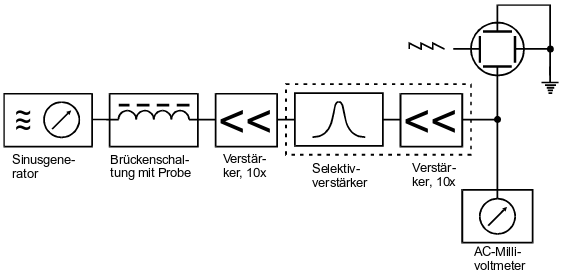
\includegraphics[scale=0.5]{Aufbau.png}
  \caption{Schematischer Versuchsaufbau\cite{anleitung}.}
  \label{abb:2}
\end{figure}
Der Schematische Versuchsaufbau ist in \ref{abb:2} dargestellt. Er besteht aus einem Sinusgenerator,
der die Brückenschaltung (vergleiche Abschnitt \ref{1.2}) speist. Das Signal der Brückenschaltung
wird um den Faktor 10 vorverstärkt und gelangt danach ein einen Selektivverstärker.
Der Selektivverstärker ist notwendig, da an der Brückenspannung multifrequente
Störsignale auftreten, von denen das monofrequente Messsignal befreit werden muss.
Im Selektivverstärker integriert ist ein weiter x10 Verstärker. Das entstörte und verstärkte
Signal kann über ein AC-\si{\milli\volt}-Meter abgelesen werden.
\subsection{Versuchsdurchführung}
In einem ersten Versuchsteil wird die Durchlasskurve des Selektivverstärkers bestimmt.
Dazu wird der Verstärker an einen Synthesizer angeschlossen. Um die Durchlassfrequenz des
Verstärkers wird die Frequenz der Synthesizerspannung variiert und die jeweils zugehörige
Ausgangsspannung gemessen.\\
\noindent
In einem zweiten Teil wird die Frequenz des Sinusgenerators auf die vorher bestimmte
Durchlassfrequenz eingestellt. Danach wird die Brückenschaltung sorgfältig auf 0 abgeglichen
und die Einstellungen der Widerstände werden notiert. Die Probe wird in die Halterung eingebracht
und die resultierende Spannungsänderung wird festgehalten. Die Schaltung wird wieder
auf 0 abgeglichen und die Werte werden notiert. Dies wird für jede Probe drei mal wiederholt.
Abschließsend werden die Proben vermessen.
\section{Auswertung}
\subsection{Untersuchung der Filterkurve}
\begin{figure}
  \centering
  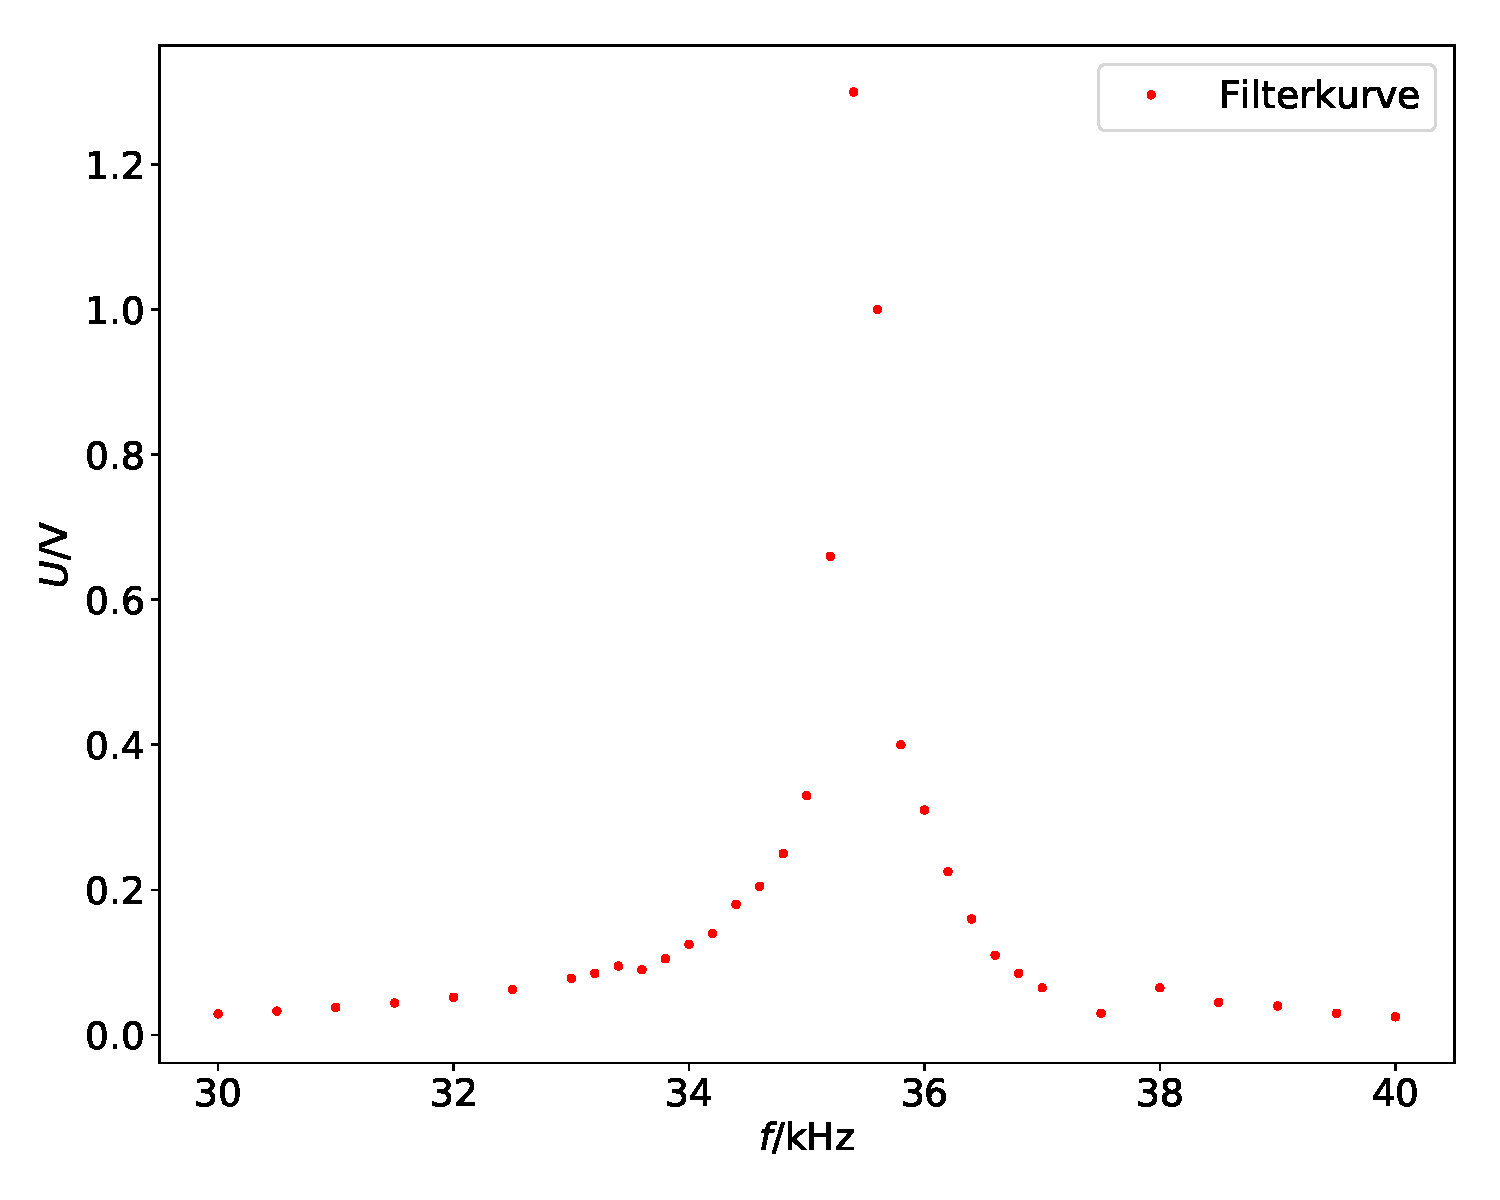
\includegraphics[scale=0.35]{filterkurve.pdf}
  \caption{Filterkurve des verwendeten Bandpasses.}
  \label{fig:1}
\end{figure}
In Abbildung \ref{fig:1} ist die Filterkurve des Bandpasses zu sehen. Das Maximum
liegt ungefähr bei \SI{35.6}{\kilo\hertz}. Dies wird beim nächsten Versuchsteil benutzt.

\subsection{Bestimmung der Suszeptibilität}
\subsubsection{Theoretische Bestimmung}
Für die Bestimmung der theoretischen Werten wird \eqref{eqn:3} genutzt. Zur Bestimmung
des Gesamtdrehimpulses $J$ und des $\textsc{Landé}$-Faktors werden die Hundschen
Regeln aus Kapitel \ref{sec:1.1} genutzt. Für die Orientierungsquantenzahl $m$ gilt
bei $l = 3$ in der 4f-Schale: (-3, -2, -1, 0, 1, 2, 3) mit  $m = 2 l + 1$. Dabei ergibt sich:
\begin{itemize}
  \item $\symup{Nd_2O_3}$ enthält 3 Elektronen in der 4f-Schale. Diese haben nach
  der ersten Hundschen Regel den gleichen Spin mit $S = \frac{3}{2}$. Da die drei Elektronen
  gleichen Spin besitzen, müssen sie sich in ihrer Orientierungsquantenzahl unterscheiden.
  Somit ergibt sich der maximale Drehimpuls zu $L = 3 + 2 +1 = 6$. Da die Schale weniger als halb
  gefüllt ist, folgt für den Gesamtdrehimpuls $J = 6 - \frac{3}{2} = 4.5$ und für den
  $\textsc{Landé}$-Faktor nach \eqref{eqn:1} $g_J = \frac{8}{11}$.

  \item $\symup{Gd_2O_3}$ hat 7 Elektronen in der 4f-Schale. Diese haben den gleichen Spin
  $S = 3.5$. Der Drehimpuls ist in diesem Fall wegen der Orientierungsquantenzahl 0.
  Damit wird der Gesamtdrehimpuls zu $J = 3.5$ und der $\textsc{Landé}$-Faktor zu $g_J = 2$.

  \item $\symup{Dy_2O_3}$ besitzt 9 Elektronen in der 4f-Schale. Da es aber nur sieben Orientierunsgquantenzahlen
  gibt, haben zwei Elektronen einen negativen Spin. Der Gesamtspin ergibt somit $S = 2.5$. Im Gegensatz
  zu $\symup{Gd_2O_3}$ beträgt der Drehimpuls somit $L = 3 + 2 = 5$. Die 4f-Schale ist mehr als halb voll
  und es folgt $J = 5 + 2.5 = 7.5$ und $g_J = \frac{4}{3}$.
\end{itemize}
Die Anzahl der Momente pro Volumeneinheit ergibt sich nach
\begin{equation}
  N = 2 \cdot N_a \frac{\rho}{M_{\symup{mol}}}
  \label{eqn:2}
\end{equation}
mit $N_a$ als Avogadro-Konstante, $\rho$\footnote{siehe \cite{anleitung}} als Dichte und $M_{\symup{mol}}$\footnote{siehe \cite{molare}} als molare Masse
des Probenmaterials.
\begin{table}
  \centering
  \caption{Konstanten zu Bestimmung von $N$.}
  \label{tab:1}
    \begin{tabular}{c c c c}
      \toprule
      & $\rho$ / \si{\gram\per\cm^3} & $M_{\symup{mol}}$ / \si{\gram\per\mol} & $N$ / \si{\per\cm\tothe{3}} \\
      \midrule
      $\symup{Nd_2O_3}$ & 7.24 & 336.48 & \num{2.59e28} \\
      $\symup{Gd_2O_3}$ & 7.40 & 362.50 & \num{2.46e28} \\
      $\symup{Dy_2O_3}$ & 7.80 & 373.00 & \num{2.52e28} \\
      \bottomrule
    \end{tabular}
\end{table}
In Tabelle \ref{tab:1} sind die Dichten und molaren Massen der verwendeten Materialen sowie
die nach \eqref{eqn:2} berechnete Anzahl pro Volumeneinheit zu finden. Damit ergeben sich für
die theoretischen Werte von $\chi$ die Werte in Tabelle \ref{tab:2}.
\begin{table}
  \centering
  \caption{Theoretische Suszeptibilitäten der drei Materialien.}
  \label{tab:2}
    \begin{tabular}{c c}
    \toprule
    & $\chi_{\symup{theo}}$ \\
    \midrule
    $\symup{Nd_2O_3}$ & \num{0.00302} \\
    $\symup{Gd_2O_3}$ & \num{0.01380} \\
    $\symup{Dy_2O_3}$ & \num{0.02541} \\
    \bottomrule
    \end{tabular}
\end{table}
\subsubsection{Bestimmung der Suszeptibilität über Widerstandsbetrachtung.}
\label{sec:r}
Die Suszeptibilität lässt sich über \eqref{eqn:4} mittels Widerstandsbetrachtung bestimmen. Der Querschnitt
der Spule beträgt \SI{86.6}{\milli\meter\tothe{2}} und für $R_3$ gilt $R_3 = \SI{998}{\ohm}$. Der Querschnitt der Probe
nach \eqref{eqn:5}, die Differenz der Widerstände und das $\chi$ befinden sich in Tabelle \ref{tab:3}.
\begin{table}
  \centering
  \caption{Querschnitt und $\Delta R$ der Probematerialien und das daraus resultierende $\chi_R$.}
  \label{tab:3}
  \begin{tabular}{c c c c}
    \toprule
    & $Q_\symup{real}$ / \si{\milli\meter\tothe{2}} & $\Delta R$ / \si{\ohm} & $\chi_R$ \\
    \midrule
    $\symup{Nd_2O_3}$ & \num{7.77}  & \num{0.16(12)} & \num{0.0037(26)} \\
    $\symup{Gd_2O_3}$ & \num{11.53} & \num{0.92(4)} & \num{0.0138(7)} \\
    $\symup{Dy_2O_3}$ & \num{12.49} & \num{1.44(4)} & \num{0.0200(5)} \\
    \bottomrule
  \end{tabular}
\end{table}
\subsubsection{Bestimmung der Suszeptibilität über Spannungsbetrachtung.}
Nach \eqref{eq:2} lässt sich $\chi_U$ berechnen mit $Q_\symup{real}$ und $F$ aus Kapitel \ref{sec:r} und einer
Saugspannung von \SI{0.9}{\volt}. Die jeweils gemessene Brückenspannung und das $\chi_U$ befinden sich in
Tabelle \ref{tab:4}.
\begin{table}
  \centering
  \caption{Brückenspannung und $\chi_U$ der Probematerialien.}
  \label{tab:4}
  \begin{tabular}{c c c}
    \toprule
    & $U_\symup{Br}$ / \si{\volt} & $\chi_U$ \\
    \midrule
    $\symup{Nd_2O_3}$ & \num{1.67(33)e-5} & \num{0.00083(17)} \\
    $\symup{Gd_2O_3}$ & \num{0.000136(18)} & \num{0.0045(6)} \\
    $\symup{Dy_2O_3}$ & \num{0.000417(12)} & \num{0.0128(4)} \\
    \bottomrule
  \end{tabular}
\end{table}

\section{Diskussion}
\begin{table}[h]
  \centering
  \caption{Theoretische und aus dem Experiment bestimmte Suszeptibilitäten.}
  \label{tab:5}
  \begin{tabular}{c c c c}
    \toprule
    & $\chi_\symup{theo}$ & $\chi_U$ & $\chi_R$ \\
    \midrule
    $\symup{Nd_2O_3}$ & \num{0.00302} & \num{0.00083(17)} & \num{0.0037(26)} \\
    $\symup{Gd_2O_3}$ & \num{0.01380} & \num{0.0045(6)} & \num{0.0138(7)} \\
    $\symup{Dy_2O_3}$ & \num{0.02541} & \num{0.0128(4)} & \num{0.0200(5)} \\
    \bottomrule
  \end{tabular}
\end{table}
In Tabelle \ref{tab:5} sind die Ergebnisse der Suszeptibilitätsbestimmung aufgelistet.
Es wird deutlich, dass die Werte aus der Bestimmung über die Widerstandsmethode nahe
an den Theoriewerten sind. $\symup{Nd_2O_3}$ und $\symup{Gd_2O_3}$ liegen innerhalb
der Messungenauigkeit, die Abweichung bei $\symup{Dy_2O_3}$ ist mit ungefähr 11$\sigma$
aber signifikant. Mögliche Gründe dafür sind Störspannungen und die Tatsache, dass
beim erneuten Abgleich die Grenze der Verschiebbarkeit des Regelwiderstandes erreicht wurde,
obwohl die Brücke noch nicht vollständig abgeglichen war. Dies erklärt die Abweichungen. \\
\\
Die Werte aus der Bestimmung über die Spannungsmethode weichen stark ab, sogar teilweise
mehrere Größneordnungen. Dies lässt sich dadurch erklären, dass die Brückenspannung
sehr sehr klein sind, damit werden die daraus errechneten Suszeptibilitäten ebenfalls
klein. Mit besseren Präzisionsmessinstrumenten wäre ein genauerer Abgleich der Brückenschaltung
und damit eine genauerer Bestimmung der Brückenspannung möglich. \\
\\
Unter dem Strich lässt sich sagen, dass vor allem die Werte, die aus der Widerstandsmethode
gewonnen wurden, überraschend gute Werte geliefert haben. Die Werte aus der Spannungsmethode
weichen stark ab, aber Abweichungen waren zu erwarten.

\newpage
\nocite{*}
\printbibliography
